\documentclass[aspectratio=169, 8pt,t]{beamer}
\graphicspath{{figures/}} % Setting the graphicspath

% Theme settings
\usetheme{Madrid}
\usecolortheme{default}
\setbeamertemplate{navigation symbols}{}   % removes navigation symbols such as 'next page'
\setbeamertemplate{footline}{}             % remove line with name, date, page nr.
\setbeamercolor*{frametitle}{bg=white}     % remove background from frametitle
\usepackage{caption}
% \captionsetup[figure]{labelformat=empty}% redefines the caption setup of the figures environment in the beamer class.
\setbeamersize{text margin left=20pt,text margin right=10pt}
\usefonttheme[onlymath]{serif} % makes beamer math look like article math
\usepackage{hyperref}

%======================= title page info =======================
\title{Methodology for NNPDF4.1 -- feature scaling}
\date{NNPDF collaboration meeting  \\[0.1cm] Amsterdam, 24 February 2024}
\author{Roy Stegeman}
\institute{\small The University of Edinburgh}


%======================= page numbering =======================
\addtobeamertemplate{navigation symbols}{}{ \usebeamerfont{footline}
  \insertframenumber / \inserttotalframenumber \hspace*{2mm} \\ \vspace*{1mm}
}


%=================================== colors ====================================
\definecolor{RoyBlue}{RGB}{22, 46, 69}
\definecolor{RoyGrey}{RGB}{64, 88, 128}

\newcommand{\hlme}[1]{{\color{red}\bf #1}} % highlight me

\setbeamercolor{structure}{fg=RoyBlue} % itemize, enumerate, etc
\setbeamercolor{frametitle}{fg=RoyGrey}
\setbeamercolor{section in head/foot}{bg=RoyBlue}


%======================= add progress dots to headline =========================
\setbeamertemplate{headline}{%
    \begin{beamercolorbox}[ht=4mm,dp=4mm]{section in head/foot}
        \insertnavigation{\paperwidth}
    \end{beamercolorbox}%
}%
\makeatother


%======================= add section title page ================================
\AtBeginSection[]{
  \begin{frame}
  \vfill
  \centering
    \usebeamerfont{title}\insertsection\par%
  \vfill
  \end{frame}
}


%=================================== titlepage =================================
\titlegraphic{\vspace*{6mm}
  
\includegraphics[height=1.5cm]{logos/edi_logo.png} \hspace{10mm}
  % 
\includegraphics[height=0.8cm]{logos/nnpdf_logo_official.pdf} \hspace{10mm}
  
\includegraphics[height=1.5cm]{logos/higgs_logo.jpg}
}

\defbeamertemplate{title page}{noinstitute}[1][]
{
  \vbox{}
  \vfill
  \begingroup
    \centering
    \begin{beamercolorbox}[sep=8pt,center,#1]{title}
      \usebeamerfont{title}\inserttitle\par%
      \ifx\insertsubtitle\@empty%
      \else%
        \vskip0.25em%
        {\usebeamerfont{subtitle}\usebeamercolor[fg]{subtitle}\insertsubtitle\par}%
      \fi%
    \end{beamercolorbox}%
    \vskip2em\par
    \begin{beamercolorbox}[sep=0pt,center,#1]{author}
      \usebeamerfont{author}\insertauthor
    \end{beamercolorbox}
  \begin{beamercolorbox}[sep=0pt,center,#1]{author}
    \usebeamerfont{institute}\insertinstitute
  \end{beamercolorbox}
  \vspace*{8pt}
  \vspace*{16pt}
    \begin{beamercolorbox}[sep=0pt,center,#1]{date}
      \usebeamerfont{date}\insertdate
    \end{beamercolorbox}\vskip0.5em
    {\usebeamercolor[fg]{titlegraphic}\inserttitlegraphic\par}
  \endgroup
  \vfill
}

\makeatletter
\setbeamertemplate{title page}[noinstitute][colsep=-4bp,rounded=true,shadow=\beamer@themerounded@shadow]
\makeatother


\begin{document}
{
\setbeamertemplate{headline}{} % remove headline from titlepage
\begin{frame}
  \titlepage
\end{frame}
}

\setbeamertemplate{enumerate items}[default]

\pgfdeclarelayer{bg}    % declare background layer
\pgfsetlayers{bg,main}  % set the order of the layers (main is the standard layer)


% SLIDES =======================================================================
\newcommand{\nn}{\vspace*{1em}}

\section*{The NNPDF model}

\begin{frame}{The NNPDF model}
  Preprocessing exists for historic reasons, it is still used to improve convergence and to model the extrapolation region. \\ \nn
  $(x,\log x)$ mixes objects with different orders of magnitude, which is poor practice from an ML standpoint \\ \nn
  $$ xf_k(x) = A_k {\color{red} x^{1-\alpha_k}(1-x)^{\beta_k}} \mathrm{NN}_k({\color{red} x,\log x}) $$

  \vspace*{0.5cm}
  \centering Can we simplify this architecture?
\end{frame}


\begin{frame}{A naive attempt}
  An obvious first attempt is $$ xf_k(x) = A_k \mathrm{NN}_k(x), $$ but this results in saturation of the activation functions:
  \begin{center}
    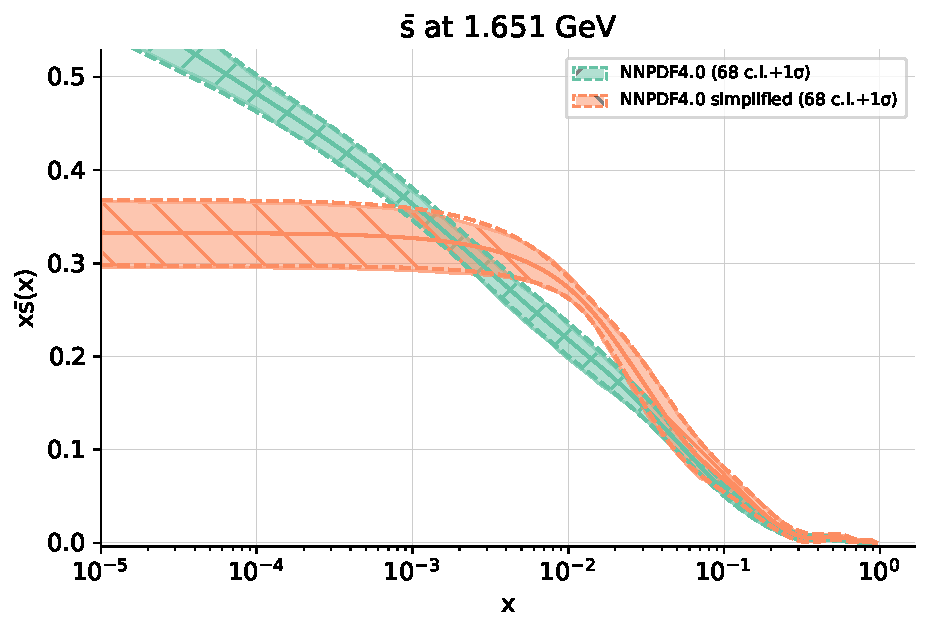
\includegraphics[height=0.55\textheight]{pdf_sbar_log_saturated.pdf}
    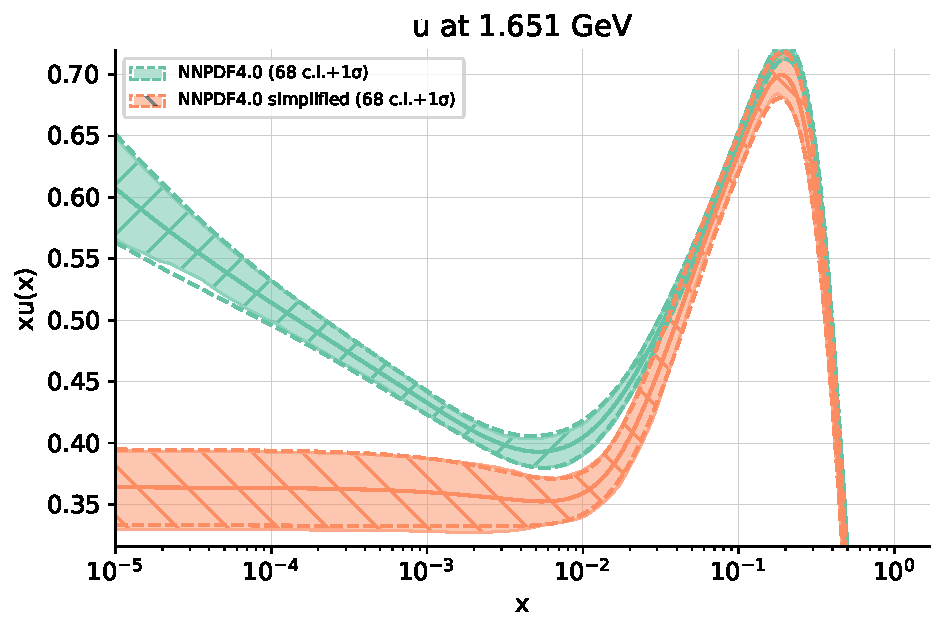
\includegraphics[height=0.55\textheight]{pdf_u_log_saturated.pdf}
  \end{center}
\end{frame}

\section*{The input}


\begin{frame}{Input}
  We can understand the small-x saturation because the optimization is not sensitive to inputs at different orders of magnitude:
  \begin{center}
    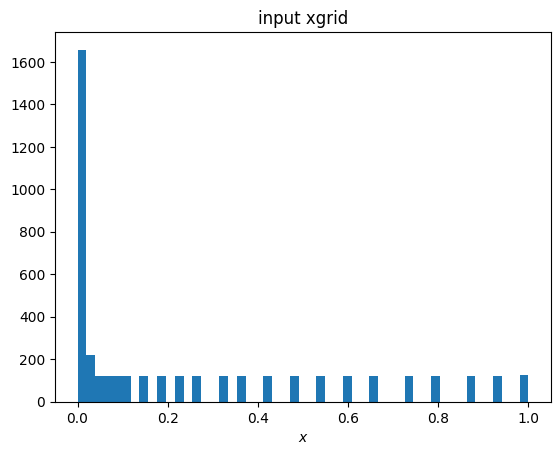
\includegraphics[height=0.55\textheight]{unscaledxgrid.png} \\
    Solution: add a second $\log(x)$ input \\
    but is this all we can do?
  \end{center}
\end{frame}

\begin{frame}{Input}
  Alternatively we can do as the ML community does and flatten the distribution following a cumulative distribution function
  \begin{center}
    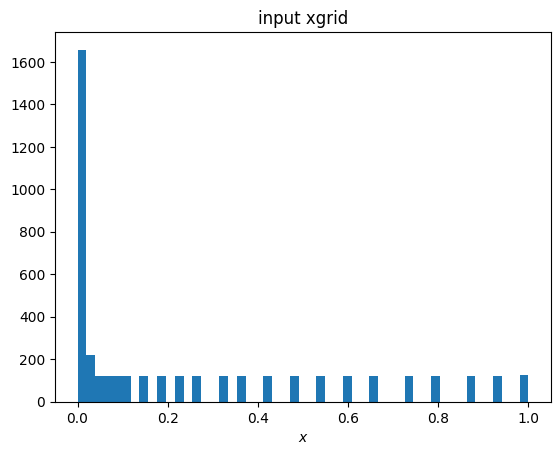
\includegraphics[height=0.55\textheight]{unscaledxgrid.png}
    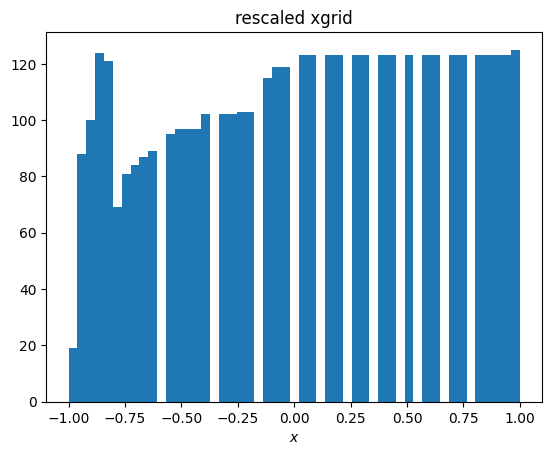
\includegraphics[height=0.55\textheight]{scaledxgrid.png}
  \end{center}
\end{frame}


\begin{frame}{results}{\url{https://vp.nnpdf.science/QrworHcxQIWe6P3rG3S3GQ==/}}
  Feature scaling \& small-x preprocessing, for large-x force $f(x=1)=0$

  \begin{itemize}
    \item Similar $\chi^2$ but larger uncertainty (as measured by $\phi$)
    \item uncertainty blows up in the extrapolation region
  \end{itemize}

  \begin{center}
    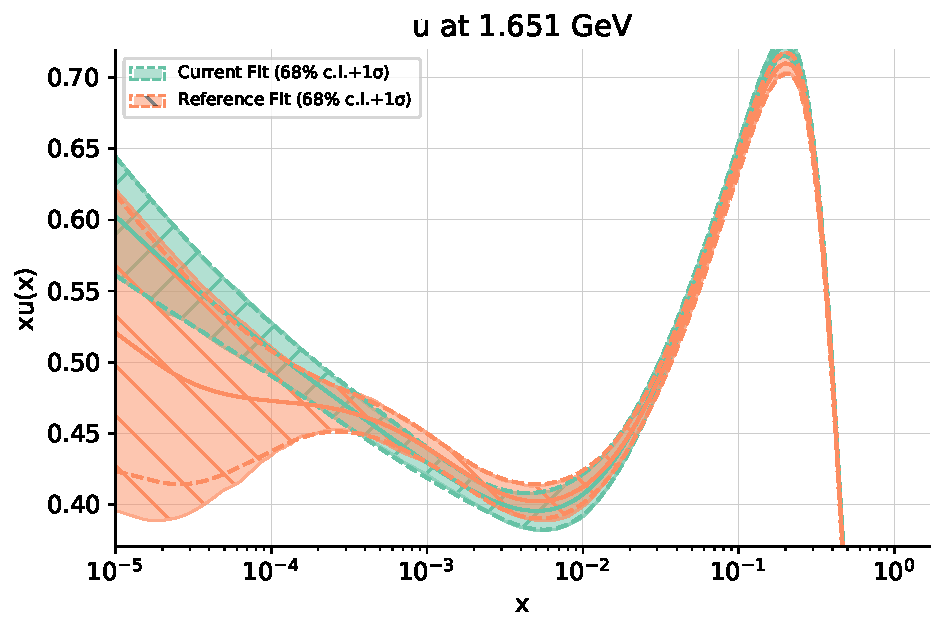
\includegraphics[height=0.55\textheight]{pdf_u_nolargexpreproc_featurescalign.pdf}
    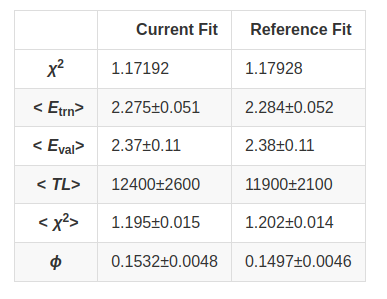
\includegraphics[height=0.55\textheight]{onlysmallxperproc_featurescaling_summary.png}
  \end{center}

\end{frame}

\section*{Preprocessing}

\begin{frame}{Preprocessing}
  Currently $\alpha_k$ and $\beta_k$ are sampled independently per replica. \\
  Alternative options are
  \begin{itemize}
    \item No preprocessing (i.e. $\alpha_k=1$, $\beta_k=0$)
    \item Make $\alpha_k$ and $\beta_k$ trainable
  \end{itemize}
\end{frame}


\begin{frame}{Results}{\url{https://vp.nnpdf.science/gBAV7UAkQUW3CnhvRA8nGQ==/}}

  Trainable preprocessing
  \begin{itemize}
    \item no improvement in $\chi^2$
    \item decreased uncertainty
    \item[$\Rightarrow$] probably still not a good idea
  \end{itemize}

  \begin{center}
    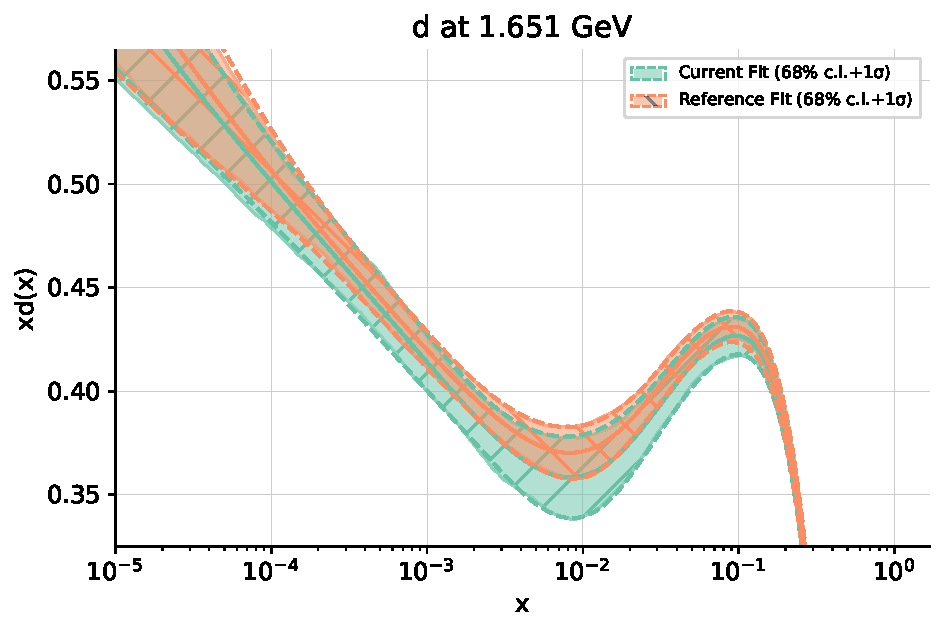
\includegraphics[height=0.5\textheight]{pdf_fittedpreproc.pdf}
    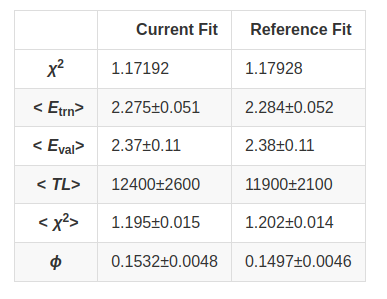
\includegraphics[height=0.5\textheight]{pdf_fittedpreproc_summary.png} \\
    current = fitted preprocessing
  \end{center}

\end{frame}


\begin{frame}{Results}{\url{https://vp.nnpdf.science/A6vFXjJJTyq4Y8Pg1MApEA==/}}
  Feature scaling no preprocessing
  \begin{itemize}
    \item Increase in uncertainty
    \item Deterioration of $\chi^2$
    \item Inputs changed with new pineline $\rightarrow$ re-hyperopt?
  \end{itemize}
  \begin{center}
    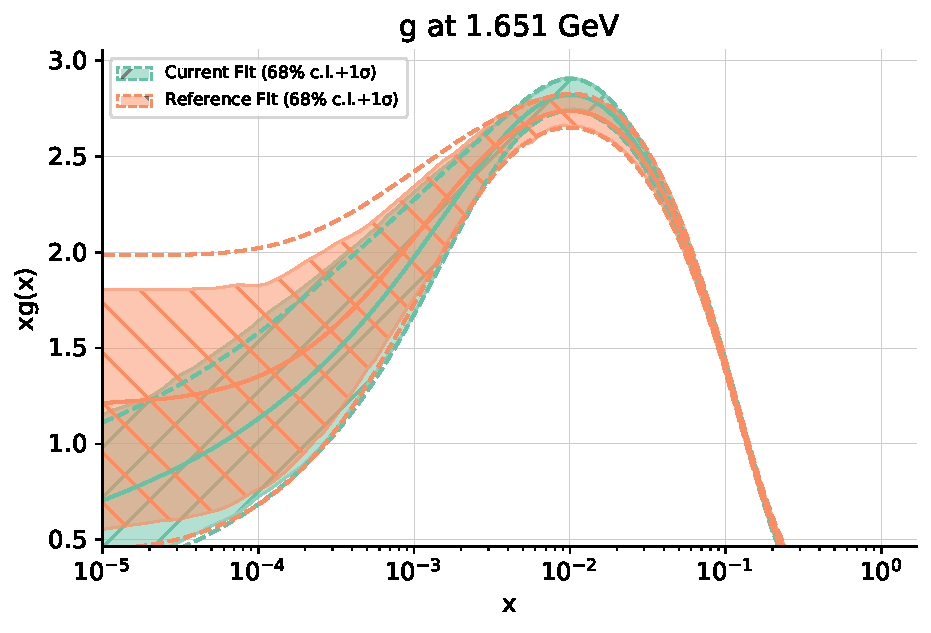
\includegraphics[height=0.5\textheight]{pdf_nopreproc_feature.pdf}
    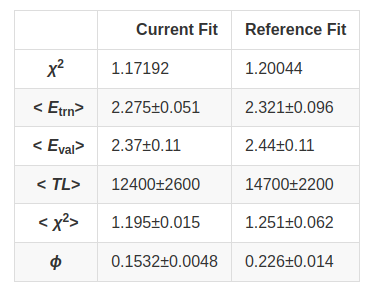
\includegraphics[height=0.5\textheight]{nopreproc_feature_summary.png} \\
  \end{center}
\end{frame}


\begin{frame}{TODO}
  Move forward in two steps \\ \vspace*{1em}

  First target: feature scaling instead of $(x,\log x)$
  \begin{itemize}
    \item Play a little more to understand the impact of the new fktable xgrids
    \item Re-hyperopt?
    \item Closure test and future test
    \item Pheno impact
    \item \ldots
  \end{itemize}

  \vspace*{1em}

  Second target: remove small-$x$ preprocessing
  \begin{itemize}
    \item Nice to remove in data region
    \item \ldots but leaves us without model for the extrapolation region
    \item Either way, requires significant tuning
  \end{itemize}
\end{frame}



\end{document}
